% header

\documentclass[10pt,a4paper]{article}
\usepackage{amsmath,mathrsfs,mathtext} 
\usepackage[latin1]{inputenc}
\usepackage{hyperref}
\usepackage{amssymb}
\usepackage{ngerman}
\usepackage{graphicx, epsfig} 
% the document
\begin{document}

% create the title
% Please replace the data in brackets [] with actual data.
\title{Abgabe - �bungsblatt [$3$]\\
\small{Einf�hrung in die Computergraphik und Visualisierung}}
\author{ [Svetlana Shishkovets] \and [Victor Lopatin] \and [Lihn Chi Tran]}
\date{\today}
\maketitle

\section*{First Exercise}
\begin{itemize}
\item (a) $p_1,p_2 \in P(\mathbb {R}^3)$\\
Remember that $(a,b,c,d)^T= (\frac{a}{d},\frac{b}{d},\frac{c}{d})^T$ if $d\neq 0, \Rightarrow$\\
$p_1=(\frac{14}{2},\frac{3}{2},\frac{4}{2}) =(7,1.5,2) $,\\
$p_2=(\frac{12}{3},\frac{0}{3},\frac{3}{3}) =(6,0,1) $ 
\item (b) Since we cannot divide by 0(otherwise we will get vector of infinite length), we cannot represent in $\mathbb {R}^3 (a,b,c,0)$ 
\end{itemize}
\section*{Second Exercise}
We will use ideas, similar to the lecture. \\
\begin{figure}[h]
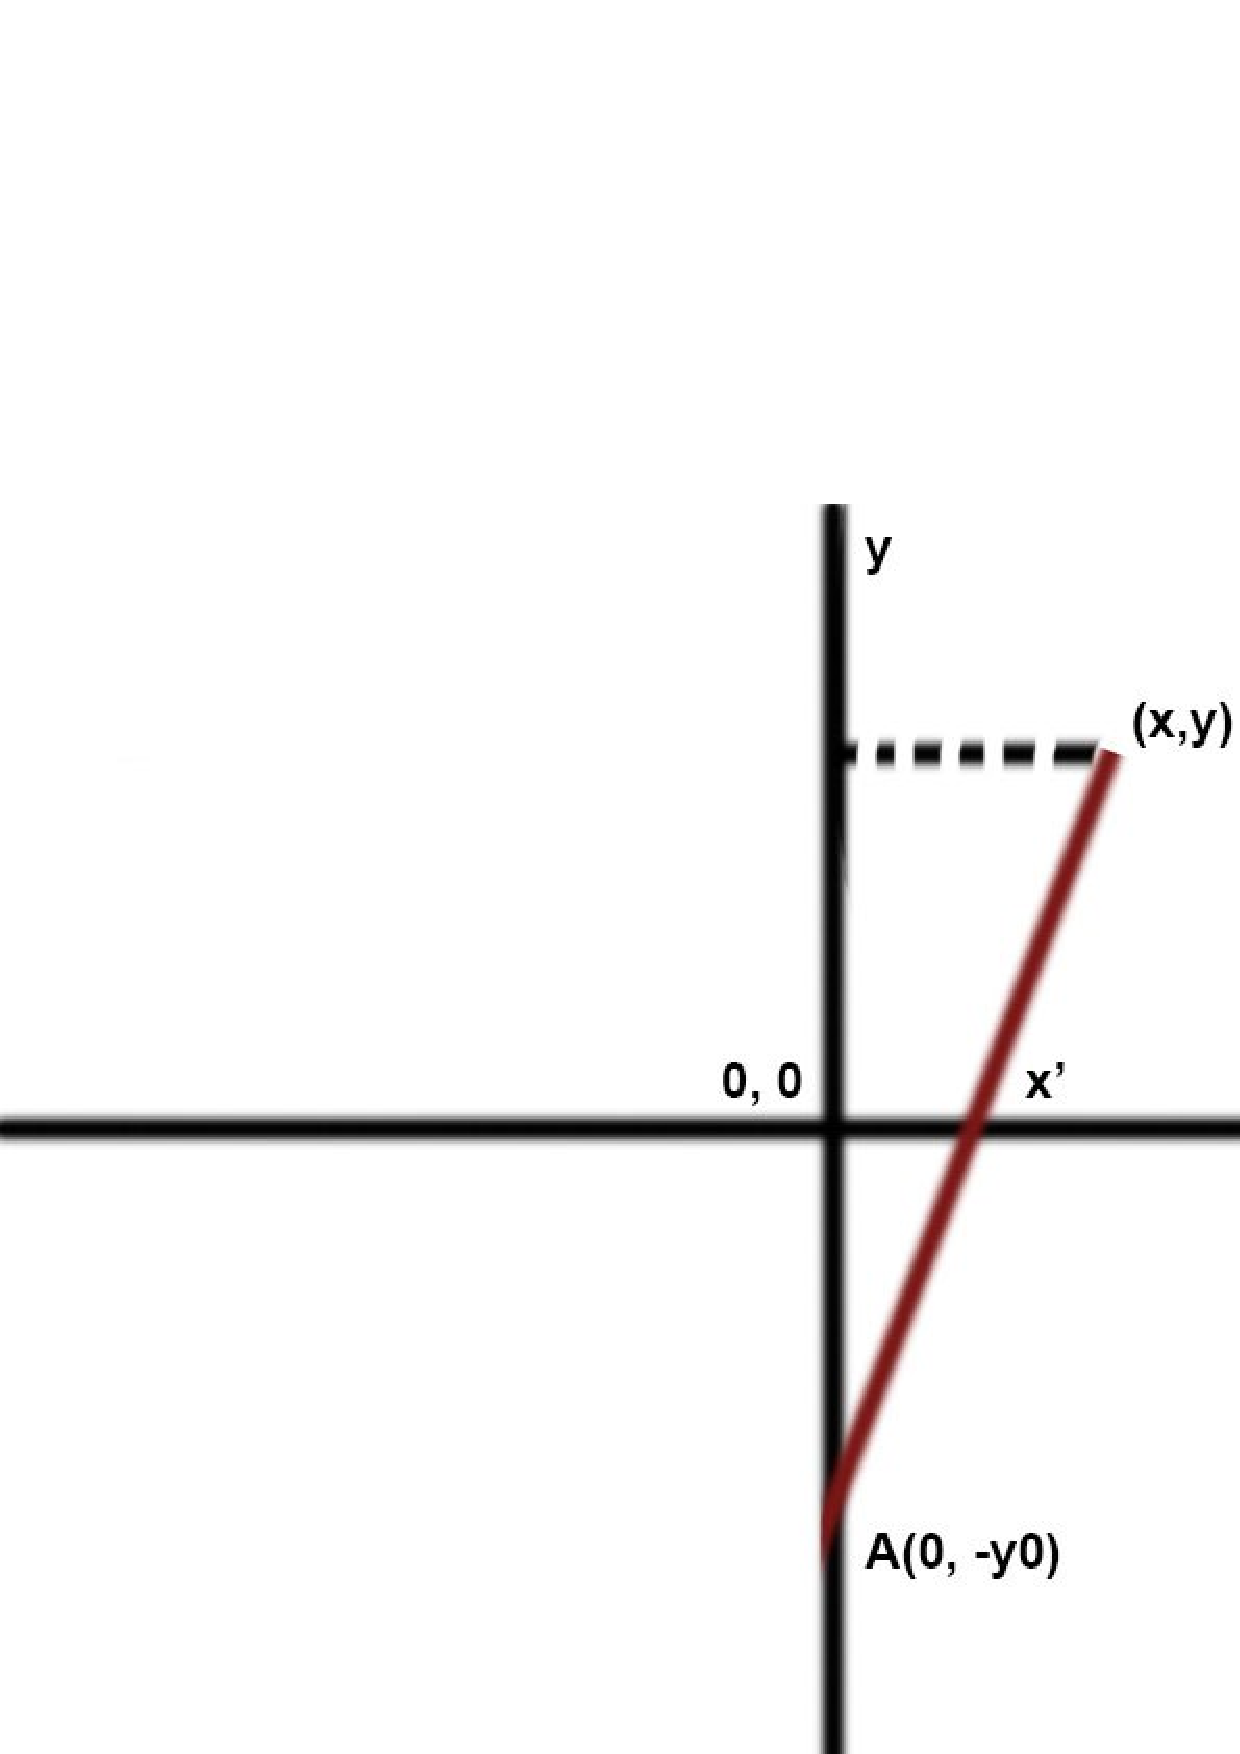
\includegraphics[scale=0.3]{1}
\end{figure}\\
$\vartriangle(A;(0; y);(x; y))\sim \vartriangle(A;(0;0);(0; x'))\Rightarrow$\\
$\frac{x'}{x}=\frac{y_0}{y+y_0} \Leftrightarrow x'=\frac{y_0x}{y+y_0}$  \\

$\begin{pmatrix}
x\\
y\\
\end{pmatrix}
\longmapsto
\begin{pmatrix}
x\\
y\\
\end{pmatrix}
-\frac{y}{y+y_0}
\begin{pmatrix}
x\\
y+y_0\\
\end{pmatrix}$\\
Let's represent with the a homogenious 3x3 matrix:\\
$\begin{pmatrix}
x'\\
y'\\
1\\
\end{pmatrix}
=
\begin{pmatrix}
y_0 & 0& 0\\
0 & 0& 0\\
0 & 1& y_0\\
\end{pmatrix}
\begin{pmatrix}
x\\
y\\
1\\
\end{pmatrix}
=
\begin{pmatrix}
1 & 0& 0\\
0 & 0& 0\\
0 & \frac{1}{y_0}&1\\
\end{pmatrix}
\begin{pmatrix}
x\\
y\\
1\\
\end{pmatrix}
$\\
We can decompose it into two mappings:  a perspective transformation followed by a parallel projection:\\
\\
$\begin{pmatrix}
1 & 0& 0\\
0 & 0& 0\\
0 & \frac{1}{y_0}&1\\
\end{pmatrix}
=
\begin{pmatrix}
1 & 0& 0\\
0 & 0& 0\\
0 & 0&1\\
\end{pmatrix}
\begin{pmatrix}
1 & 0& 0\\
0 & 1& 0\\
0 & \frac{1}{y_0}&1\\
\end{pmatrix}
$\\
Where left matrix is parallel projection and right perspective transformation.
\end{document}
